\section{Fundamentals}
\subsection{NTDS.DIT}
\index{Active Directory!NTDS}
\label{win:NTDS}

The NTDS.DIT file can be considered the heart of Active Directory. It is stored
on a Domain Controller at \verb+C:\Windows\NTDS\+ and is a database that stores
AD data such as information about user and group objects, group membership,
and, most important to attackers and penetration testers, the password hashes
for all users in the domain. Once full domain compromise is reached, an
attacker can retrieve this file, extract the hashes, and either use them to
perform a pass-the-hash attack or crack them offline using a tool such as
Hashcat to access additional resources in the domain. If the setting Store
password with reversible encryption is enabled, then the NTDS.DIT will also
store the cleartext passwords for all users created or who changed their
password after this policy was set. While rare, some organizations may enable
this setting if they use applications or protocols that need to use a user's
existing password (and not Kerberos) for authentication.


\subsection{Global Uniqque ID (GUID)}
objects have a globally unique identifier (GUID) assigned to them by the system
at creation. This 128-bit number is the Microsoft implementation of the
universally unique identifier (UUID) concept from Digital Equipment
Corporation.

The object’s GUID stays with the object until it is deleted, regardless of
whether it is renamed or moved within the directory information tree (DIT). The
ob‐ ject’s GUID will also be preserved if you move an object between domains
within a multidomain forest.

\subsection{Domain and Domain Tree}
Active Directory’s logical structure is built around the concept of domains. 

An Active Directory domain is made up of the following components:
\begin{itemize}
    \item  An X.500-based hierarchical structure of containers and objects
    \item  A DNS domain name as a unique identifier
    \item  A security service, which authenticates and authorizes any access to
        resources via accounts in the domain or trusts with other domains
    \item  Policies that dictate how functionality is restricted for users or
        machines within that domain
\end{itemize}

A domain controller (DC) can be authoritative for one and only one domain. It
is not possible to host multiple domains on a single DC.

{\bf Domain tree} is a series of domains connected together in a hierarchical
fashion, all using a contiguous naming scheme.

A domain tree is called by the name given to the root of the tree

Trees ease management and access to resources, as all the domains in a domain
tree trust one another implicitly with transitive trusts.

\subsection{Forest}
A {\bf forest} is a collection of one or more domain trees.

These domain trees share a common {\bf Schema} and {\bf Configuration
container}, and the trees as a whole are connected together through transitive
trusts.

A forest is named after the first domain that is created, also known as the
forest root domain.


\subsection{Trusts}
\label{active-directory:trust}

An Active Directory (AD) Forest is the security and administrative boundary for
objects and entities.
\href{https://social.technet.microsoft.com/wiki/contents/articles/50969.active-directory-forest-trust-attention-points.aspx}{trust}
is used to establish \verb+forest-forest+ or \verb+domain-domain+
authentication, allowing users to access resources in (or administer)  another
domain outside of the domain their account resides in. A trust  creates a link
between the authentication systems of two domains.

There are several trust types:

\begin{tabularx}{\linewidth}{|l|X|}
    \hline
Trust Type & Description \\
    \hline
Parent-child & Domains within the same forest. The child domain has a two-way
transitive trust with the parent domain. \\
    \hline
Cross-link & a trust between child domains to speed up authentication. \\
    \hline
External & A non-transitive trust between two separate domains in separate
forests which are not already joined by a forest trust. This type of trust
utilizes
\href{https://www.serverbrain.org/active-directory-2008/sid-history-and-sid-filtering.html}{SID
filtering}. \\
    \hline
Tree-root & a two-way transitive trust between a forest root domain and a new
tree root domain. They are created by design when you set up a new tree root
domain within a forest. \\
    \hline
Forest & a transitive trust between two forest root domains.\\ 
    \hline
\href{https://docs.microsoft.com/en-us/security/compass/esae-retirement}{ESAE}
    & A bastion forest used to manage Active Directory which is becoming
    obsolete\\
\end{tabularx}

\begin{figure}
  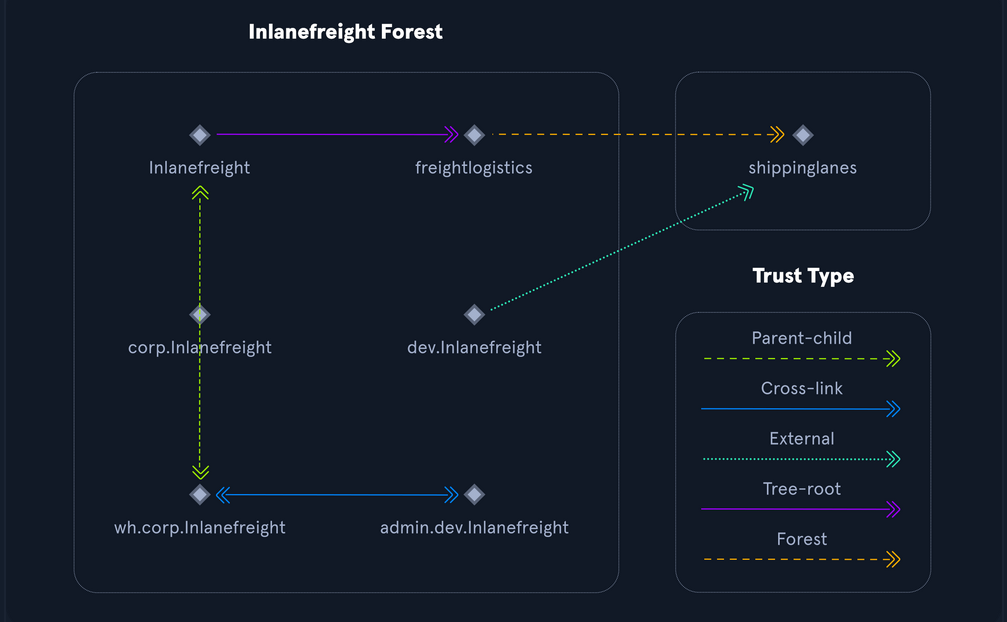
\includegraphics[width=\linewidth]{ad/knowledge/images/trusts.png}
  \caption{AD trusts}
  \label{fig:ad-trusts}
\end{figure}

Trusts can be:
\begin{itemize}
\item transitive: trust is extended to objects that the child domain trusts.
\item non-transitive: only the child domain itself is trusted.
\end{itemize}


Trusts can be set up:
\begin{itemize}
    \item bidirectional: users from both trusting domains can access resources.
    \item In a one-way trust: only users in a trusted domain can access resources in a trusting domain, not vice-versa. The direction of trust is opposite to the direction of access.
\end{itemize}

Often, domain trusts are set up improperly and provide unintended  attack
paths. Also, trusts set up for ease of use may not be reviewed  later for
potential security implications. Mergers and acquisitions can  result in
bidirectional trusts with acquired companies, unknowingly  introducing risk
into the acquiring company's environment. It is not  uncommon to be able to perform an attack such as Kerberoasting against a  domain outside the principal domain and obtain a user that has  administrative access within the principal domain.


